% Figure 16 -- step 1 / step 2 quivers and the quiver tail of the regular singularity
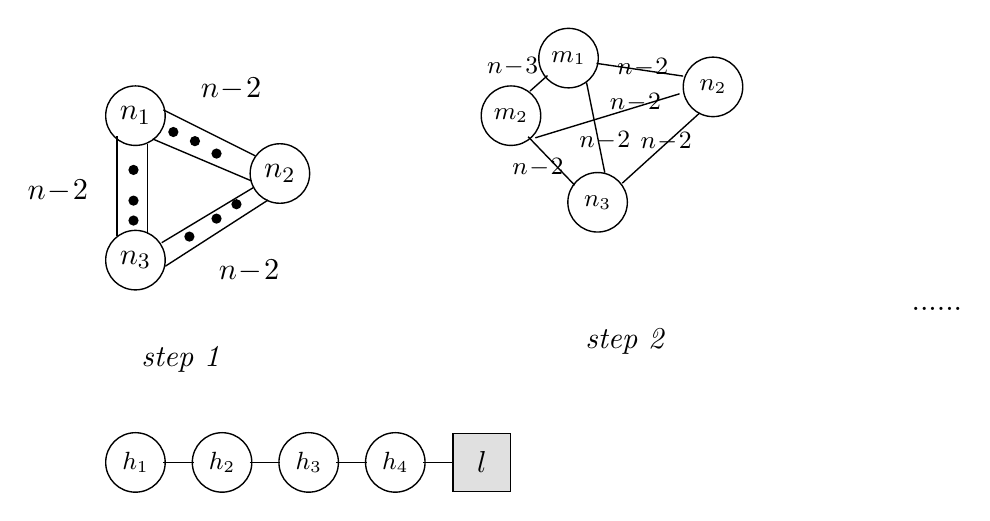
\begin{tikzpicture}[x=1pt,y=1pt,>=stealth,line width=0.5pt,
   circ/.style={circle,draw,minimum size=21.5pt,inner sep=0pt}]
  \def\rr{1.85}
  % ======================== step 1 ========================
  % --- n1--n3 ribbon ---
  \draw (50.1,104.0) -- (50.1,140.1);
  \draw (61.2,105.0) -- (61.2,137.5);
  \foreach \y in {384.0,395.1,402.3} {\fill (56.1,{512-\y}) circle[radius=\rr pt];}
  % --- n1--n2 ribbon ---
  \draw (63.0,139.2) -- (98.8,124.0);
  \draw (66.9,149.7) -- (100.1,133.1);
  \fill (70.5,141.7) circle[radius=\rr pt];
  \fill (78.3,138.4) circle[radius=\rr pt];
  \fill (86.1,133.9) circle[radius=\rr pt];
  % --- n3--n2 ribbon ---
  \draw (66.3,101.7) -- (99.4,121.6);
  \draw (67.6,93.2) -- (104.7,117.1);
  \fill (76.3,103.9) circle[radius=\rr pt];
  \fill (86.1,110.4) circle[radius=\rr pt];
  \fill (93.3,115.6) circle[radius=\rr pt];
  % ======================== step 2 ========================
  \draw (199.4,156.5) -- (205.7,162.1);
  \draw (223.4,166.5) -- (254.7,161.9);
  \draw (219.8,159.6) -- (226.4,127.0);
  \draw (198.7,140.0) -- (215.5,122.5);
  \draw (201.3,139.6) -- (253.4,155.5);
  \draw (232.7,123.2) -- (260.5,148.4);
  % ======================== nodes ========================
  \node[circ] (n1) at (56.8,147.6)   {\fontsize{11}{13}\selectfont$n_1$};
  \node[circ] (n2) at (109.0,126.7)  {\fontsize{11}{13}\selectfont$n_2$};
  \node[circ] (n3) at (56.8,95.4)    {\fontsize{11}{13}\selectfont$n_3$};
  \node[circ] (mm1) at (213.3,168.4) {\fontsize{9}{11}\selectfont$m_1$};
  \node[circ] (mm2) at (192.5,147.6) {\fontsize{9}{11}\selectfont$m_2$};
  \node[circ] (sn3) at (223.8,116.3) {\fontsize{9}{11}\selectfont$n_3$};
  \node[circ] (sn2) at (265.5,158.0) {\fontsize{9}{11}\selectfont$n_2$};
  % ======================== quiver tail ========================
  \draw (66.8,22.3) -- (77.9,22.3);
  \draw (98.1,22.3) -- (109.2,22.3);
  \draw (129.4,22.3) -- (140.5,22.3);
  \draw (160.8,22.3) -- (171.6,22.3);
  \draw[fill=black!12] (171.6,11.9) rectangle (192.4,32.8);
  \node[circ] (h1) at (56.8,22.3)  {\fontsize{9}{11}\selectfont$h_1$};
  \node[circ] (h2) at (88.1,22.3)  {\fontsize{9}{11}\selectfont$h_2$};
  \node[circ] (h3) at (119.4,22.3) {\fontsize{9}{11}\selectfont$h_3$};
  \node[circ] (h4) at (150.7,22.3) {\fontsize{9}{11}\selectfont$h_4$};
  \node[inner sep=0pt] at (182.0,22.35) {\fontsize{11}{13}\selectfont$l$};
  % ======================== labels ========================
  \node[inner sep=0pt] at (91.35,157.35) {\fontsize{11}{13}\selectfont$n\!-\!2$};
  \node[inner sep=0pt] at (97.85,91.55)  {\fontsize{11}{13}\selectfont$n\!-\!2$};
  \node[inner sep=0pt] at (28.75,120.25) {\fontsize{11}{13}\selectfont$n\!-\!2$};
  \node[inner sep=0pt] at (193.1,165.5)  {\fontsize{9}{11}\selectfont$n\!-\!3$};
  \node[inner sep=0pt] at (240.1,164.85) {\fontsize{9}{11}\selectfont$n\!-\!2$};
  \node[inner sep=0pt] at (237.45,152.45){\fontsize{9}{11}\selectfont$n\!-\!2$};
  \node[inner sep=0pt] at (226.4,138.75) {\fontsize{9}{11}\selectfont$n\!-\!2$};
  \node[inner sep=0pt] at (248.55,138.1) {\fontsize{9}{11}\selectfont$n\!-\!2$};
  \node[inner sep=0pt] at (202.25,129.0) {\fontsize{9}{11}\selectfont$n\!-\!2$};
  \node[inner sep=0pt] at (73.1,59.55)   {\fontsize{11}{13}\itshape step 1};
  \node[inner sep=0pt] at (233.55,66.05) {\fontsize{11}{13}\itshape step 2};
  \node[inner sep=0pt] at (346.4,77.85)  {\fontsize{11}{13}\selectfont......};
\end{tikzpicture}
